\documentclass[11pt]{article}

\usepackage{alltt,fullpage,graphics,color,epsfig,amsmath, amssymb}
\usepackage{hyperref}
\usepackage{boxedminipage}
\usepackage[ruled,vlined]{algorithm2e}
\usepackage{amsmath}
\usepackage{commath}
\usepackage{graphicx}
\graphicspath{ {.} }
\newcommand{\floor}[1]{\lfloor #1 \rfloor}
\newcommand{\ceil}[1]{\lceil #1 \rceil}
\title{CS 512 Midterm}
\author{Daniel Campos}
\date{March 15th,2021}
\begin{document}
\maketitle
\section{Short Questions}
\subsection{If we train a classifier with few training samples then the classifier is less likely to overfit}
\textbf{False}. A smaller dataset is more easily skewed from the true data distribution than a larger one and as a result a classifier trained on a smaller sample of data is \textit{more} likely to overfit
\subsection{Self-training does not require labeled data}
\textbf{False}. Labeled data is required to train the initial classifier which then can perform self-training on the larger unlabeled data sample.
\subsection{Transfer learning is effective when the source and target task share many common grounds}
\textbf{True}. Take for example NLP or computer vision, effective transfer learning happens when the pretraining corpus resembles the fine tuning corpus. For computer vision is the structure of images, for NLP its the structure of language. 
\subsection{The results of two runs of K-means algorithm on the same dataset are expected to be the same regardless of different initialization.}
\textbf{False}. Initialization will completely skew what kind of results are found, popular methods like Forgy choose random points to be the centroids while Random Partition tends to chose points close to the data centroid. 
\subsection{In a transaction database, if the absolute support of the itemset X is larger than the absolute support of the itemset Y, then the relative support of the itemset X must be larger than the relative support of the itemset Y}
\textbf{True}. $support_{relative}(X) = (|X|/|T|)*100 ?= support_{relative}(Y) = (|Y|/|T|)*100$? Since $support_{abs}(X) = |X|,  support_{abs}(Y) = |Y|$ and $support_{abs}(X) > support_{abs}(Y)$ it implies $|X| > |Y|$ which since the transaction database size, $|T|$, is constant implies $support_{relative}(X) > support_{relative}(Y)$
\subsection{Explain why random walk with restart (RWR) is a good measure for node proximity in terms of catching information from both short and long distance?}
RWR is a good measure because it essentially measure the probability of reaching a given node from a start node. Since the algorithm has restarts we can discover long distance connections which can only be found by restarting and walking down a different path. 
\subsection{In frequent graph pattern mining, what is major computational cost for pattern growth approach? List one solution for this challenge.}
Since the algorithm finds patterns by building from the bottom up for long sequences this can have major overhead in memory. For example, if the target pattern is of length 100 then we must generate and store about $10^30$ candidates. Additionally, at each step of the algorithm we must scan the entire database which can be quite computationally expensive. To avoid the cost of scanning the entire database each time strategies like partitioning the database and using database projections. 
\subsection{What is the key difference between active learning and transductive learning?}
In transductive learning the amount of labeled data points does not change while in active learning the most salient points are sampled for human labeling. 
\subsection{After training for an SVM classifier is done, how is the testing/evaluation performed given a new data sample $x'$}
First, when we get the new data sample we should split it into equal portions of evaluation/validation to ensure we do not overfit based on our validation. Then, for each class in our classifier we rewrite each class specific MMH using the Lagrangian formulation to rewrite the decision boundary of our SVM as $d(X) = \sum_{i=1}^l y_i \alpha_i X'x_i+b$. We plug our test dataset and check to see the sign of the result, if its negative it is not in the class and if it is positive its in the class. We run this on the entire validation/evaluation set and we check what the precision and recall of correct class is across tasks.
\subsection{In Gaussian mixture model, how to alleviate the problem of local optima}
The problem of local optima can be overcome by running the algorithm multiple times with random initialization. 
\section{Frequent Pattern Mining}
\subsection{Transnational}
\subsubsection{Frequentset}
frequent set with support: A(0.6), B(0.6), D(1), E(0.8), F(0.6), AD(0.6), BD(0.6), BE(0.6), DE(0.8), DF(0.6),BED(0.6),
\subsubsection{Strong Association Rules}
The only strong association rules are BD $\rightarrow$ E, BE $\rightarrow$ D. 
\subsection{Sequence}
\subsubsection{Projected database for <b> and <j>}
for $<b>$:(bde)(be)gj(em), (\_g)e(de)j(bj), (\_dg)gmed, EMPTY, (\_em)(edj)bd . \\
for $<j>$: (em), (bj), (\_m)(bdg)gmed, EMPTY, (\_)bd
\subsubsection{Support}
$<bej>=0.4, <mdg>=0.2, <mbj>=0.0$
\subsection{Graph}
\subsubsection{Let min\_support = 0.6, find all all frequent patterns with size $K > 2$}
First, we start with all patterns k=1 where we get: H:5, O:5, C:5, S:2 and we drop s. \\
Next, we find all patterns k=2 and we get: H-O:5, O-H:5, H-H:1, H-C:4, C-H:4, C=O:4, O=C:4, O-C:5, C-O:5 and we drop H-H \\
Moving to patterns of k> 2 and confidence >= 0.6: \textbf{O-C=O(Support 0.8), O-C-H(0.6), H-C-O(0.6), H-C-H(0.6), H-O-C(0.8)} and all re orderings of the mentioned examples. 
\subsubsection{Let min\_confidence = 0.7 and min\_support = 0.6. List one strong association rule and the corresponding confidence. }
The association rule we find is O=C $\longrightarrow$ O=C-O as both O=C and O=C-O have a confidence of 0.8 and thus the confidence in association = 1
\section{SVM}
\subsection{If there is a mapping of $R^1 \rightarrow R^2$ by which the mapped positive and negative data samples can be linearly separable? Plot the data points after mapping in 2-d space}
Yes There does exist see figure \ref{fig:svm1}
\begin{figure}[]
\centering
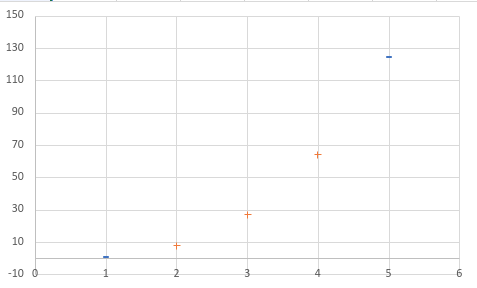
\includegraphics[width=12cm]{Assignments/MidTerm/svmpart1.png}
\caption{Liberally separating data part 1}
\label{fig:svm1}
\end{figure}
\subsection{If we implement a hard margin linear SVM on the mapped data samples from problem A what is the decision boundary? Draw it on your figure and mark the corresponding support vectors.}
As shown in figure \ref{fig:svm2} our separation runs right along the two classes and is a the blue line is the support vector for $-$ and the orange line is the support vector for $+$
\begin{figure}[]
\centering
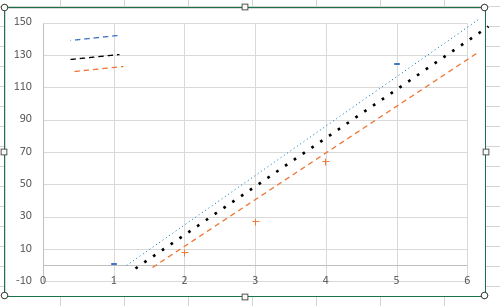
\includegraphics[width=12cm]{Assignments/MidTerm/svmpart2.png}
\caption{Liberally separating data part 1}
\label{fig:svm2}
\end{figure}
\subsection{What is the corresponding kernel $K(x_1, x_2)$}
The kernel I implemented was $K(x_1, x_2) = x, x^3$
\subsection{Does there exist a mapping $R^1 \rightarrow R^2$ such that mapped points can be linearly separable? Plot the points after mapping to a 2-d space}
Yes there does exist a linearly separable space as shown by figure \ref{fig:svm3}. For this data my kernel was $k(x_1, x_2) = x, (\sin(x_1)+4)$
\begin{figure}[]
\centering
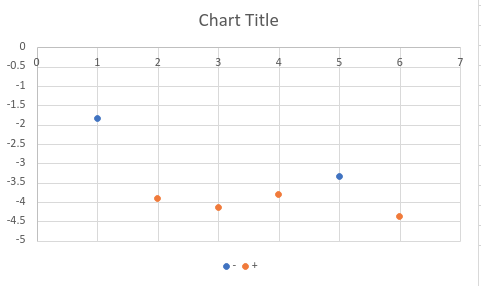
\includegraphics[width=12cm]{Assignments/MidTerm/svmpart3.png}
\caption{Liberally separating data part 3}
\label{fig:svm3}
\end{figure}
\section{Random Walk with Restart}
\subsection{Adjacency matrix A of Network G}
See table \ref{tab:adj1}
\begin{table}[]
\begin{tabular}{|l|l|l|l|l|l|} \hline
1 & 1 & 1 & 0 & 0 & 0 \\ \hline
1 & 1 & 1 & 1 & 0 & 1 \\ \hline
1 & 1 & 1 & 1 & 0 & 0 \\ \hline
0 & 0 & 0 & 1 & 1 & 1 \\ \hline
0 & 0 & 0 & 1 & 1 & 1 \\ \hline
0 & 1 & 0 & 1 & 1 & 1  \\\hline
\end{tabular}
\caption{adjacency matrix A of network G}
\label{tab:adj1}
\end{table}
\subsection{Row normalized adjacency matrix}
See table \ref{tab:adj2}
\begin{table}[]
\begin{tabular}{|l|l|l|l|l|l|}
\hline
.33 & .33 & .33 & 0   & 0   & 0   \\ \hline
.2  & .2  & .2  & .2  & 0   & .2  \\ \hline
.25 & .25 & .25 & .25 & 0   & 0   \\ \hline
0   & 0   & 0   & .33 & .33 & .33 \\ \hline
0   & 0   & 0   & .33 & .33 & .33 \\ \hline
0   & .25 & 0   & .25 & .25 & .25 \\ \hline
\end{tabular}
\caption{row normalized adjacency matrix A of network G}
\label{tab:adj2}
\end{table}
\subsection{What node is the most relevant to node 2 using the RWR formula. Report Results of the first three iterations.}
The first iteration gives us node 0 with a value of 0.40. The second iteration gives us node 0 with the value 0.22. The third iteration gives us node 0 with a value of 0.17. 
\section{K-Means}
\subsection{What is the Manhattan distance between A and E}
The distance is 7.
\subsection{Run K means for 2 iterations using 2 centroid with initialization of (0, -3) and (2, -2)}
For iteration 1 centroid 1 is: (0,-3) and centroid 2 is: (2,-2) and A,C, D belong to centroid 1 while B and E belong to centroid 2. \\
For iteration 2 centroid 1 is: (-1.33, 0) and centroid 2 is: (1.5, -0.5) and A,C belong to centroid 1 while B, D, E belong to centroid 2. \\
For iteration 3 centroid 1 is : (-2.0, 1.5) and centroid 2 is: (1.0, -1.33) and A, C belong to centroid 1 while B,D, E belong to centroid 2. After this iteration the algorithm converges. 
\subsection{Has the K-means converged in the first 3 iterations on the provided data? Why? }
Yes it has. It has converged because after iteration 2 the data points in each cluster do not change which means the centroids chosen for iteration 3 do not change no matter how many more iterations we run. 
\subsection{How many possible different clustering are there}
Since K means is so heavily dependent on initialization point there are theoretically infinite combinations of possible centroid(assuming centroids do not have to be integers). If we limit the question to how many ways can our 5 points be arranged into 2 clusters by k means there are a few essential combinations which to combine: 4 in cluster 1 and 1 in cluster 2, 3 in cluster 1 and 2 in cluster 2, 2 in cluster 1 and 3 in cluster 2, 1 in cluster 1 and 4 in cluster two. We can rewrite this as a combinatorial problem $number-clustering=\frac{5!}{2!}{3!}*2+\frac{5!}{4!}{1!}*2= \frac{2*120}{2*6} + \frac{2*120}{24}= \frac{240}{12} + \frac{240}{24} = 20 + 10 = 30$. There are 30 possible clusters.
\section{2-way spectral graph partitioning}
\subsection{Explain why the mincut loss function can be formulated as $J = \frac{1}{4}\sum_{i,j} (q[i] - q[j])^2 A[i,j]$}
The loss function is formulated by the formula above because it is the most efficient way to represent how far off the connected graph is from the associated class. The $\frac{1}{4}$ is to normalize for when classes disagree since if $q_i = 1$ and $q_j=-1$ $(q_i-q_j)^2 = (1-(-1))^2= 2^2 = 4$ so we divide the summation by 4. We sum over all i, j because we want to compare every node in the graph. The main loss function $(q_i - q_j)^2$ is standard to loss(error squared). Finally we multiply by the adjacency matrix because we only care about any error if the nodes are connected in our adjacency matrix. If nodes are not connected but disagree on class this does not effect out loss. 
\subsection{Prove the loss function of MinCut can be rewritten as $J= \frac{1}{2}q^T(D-A)q$}
Since the original formulation is NP hard we relax $q_i$ from being either -1 or 1 to being any real number between -1 and 1. We then impose the constraint $\sum_{i=1}^n q_i^2= n$ as we must make the total membership vector equal to the amount of nodes in the graph.\\
First we simplify, $J = \frac{1}{4}\sum_{i,j} (q[i] - q[j])^2 A[i,j] = \frac{1}{4}\sum_{i,j} q[i]^2 + q[j]^2 - 2q_i q_j A[i,j]$. // 
Since $d_i = \sum{j}w_{i,j}$ we then further simplify $J = \frac{1}{4}\sum_i 2q_i^2 (d_i) - \frac{1}{4} \sum_{i,j}2q_i*q_j*w_{i,j}$ //
Then $J=\frac{1}{2}\sum q_i^2*d_i - \frac{1}{2}\sum_{i,j}q_i * q_j* w_{i,j} = \frac{1}{2} \sum_i q_i(d_i, \gamma_{i,j}  - w_{i,j}q_j$. Which since we know that $D= [d_i \gamma_{i,j}$ we arrive at our intended $J= \frac{1}{2} *q^\textbf{T}(D-W)q$
\subsection{Explain why we need to relax the constrain from $q \in {-1, 1}^N$ to $\sum (q_i)^2 = n$}
We need to relax this because when values in q can only be -1 or 1 the problem is NP hard as we must explore the entire space. Additionally by moving away from this 2 class distribution we must impose the total vertex constraint to prevent from having too many nodes that w
\subsection{Why can we not select the eigenvector corresponding to the minimum eigenvalue to do the 2-way cut}
We cannot select the smallest eigenvector because when we have a graph laplacian multiplication the smallest eigenvalue will be 0 which will mean the smallest eigen vector will have all vector values be set to $\frac{1}{n}$. To avoid this problem we choose the second smallest eigenvalue and related the second smallest eigenvector.
\subsection{What happens if we change the mincut constraint from n to 10n}
If we increase the N value we are increasing the size of the minimum cuts we have to do to separate the graph. A larger constant will mean that more items that are connected need to be in one of the two classes which in turn will cut the graph further. This will make the solution less optimal because we are not minimizing the amount of cuts we need to make. We are essentially increasing the amount of cuts required by $\sqrt{10}$ since we are requiring the membership vector to have that many more non zero values in it. 
\end{document}